\textbf{(3)} Considere o sistema representado abaixo, onde um compartimento de
volume V, dividido em dois volumes de \num{0,25} V e um de \num{0,50} V. Um dos volumes
menores foi preenchido com \num{0,75} mols de \ce{N2} e o outro dos volumes menores com
\num{0,25} mols de \ce{O2}, ambos a 300 K, como ilustrado abaixo. Em um certo momento, a
barreira que divide o volume é removida.  Considere ainda que os gases são
ideais.\\

\begin{figure}[H]
    \centering
    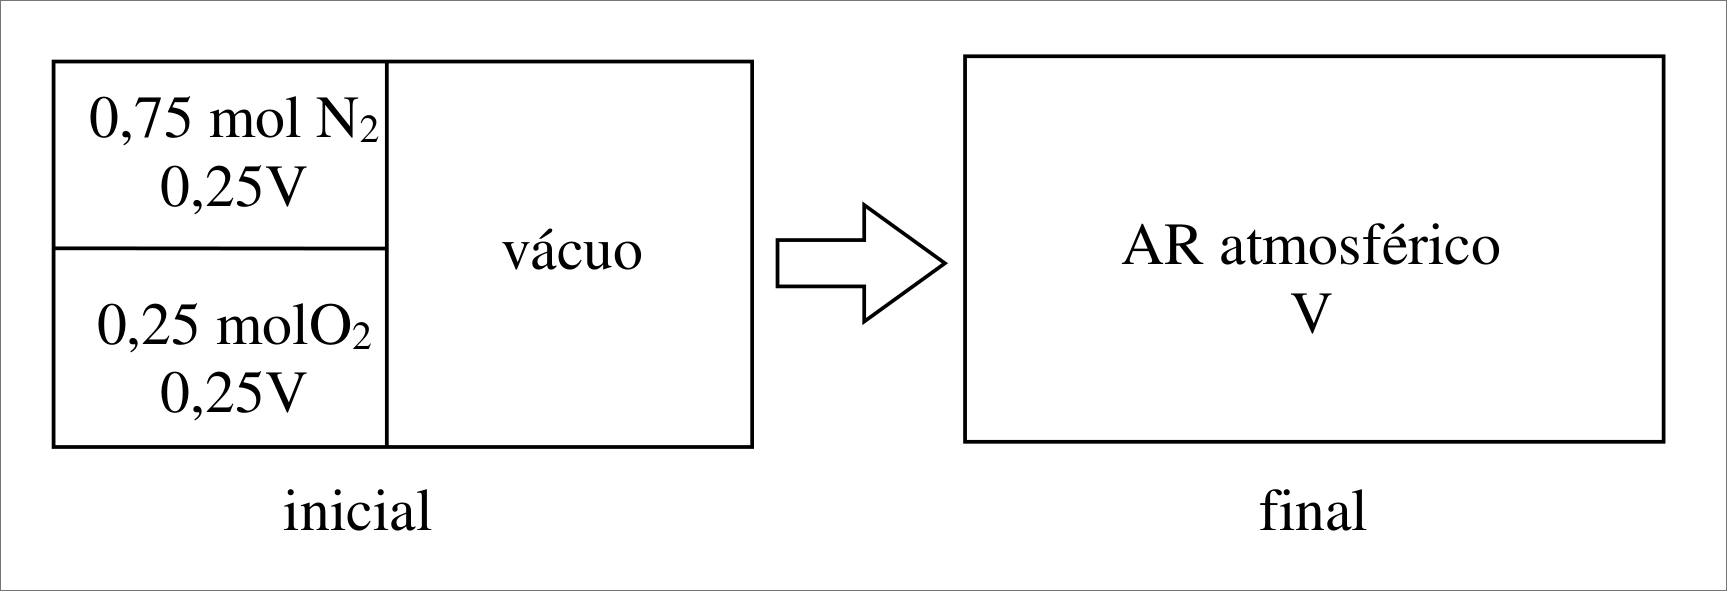
\includegraphics[width=.8\linewidth]{Q3.png}
\end{figure}

(a) Calcule a variação de entropia do \ce{N2} e do \ce{O2} entre os estados
final e inicial sabendo que a temperatura permanece constante. Indique os
cálculos a partir da derivada total apropriada.\\

(b) Calcule a variação de entropia total do sistema entre o estado inicial e
final (após a remoção das divisórias).\\

(c) Explique porque a mistura de \ce{O2} e \ce{N2}, nas condições descritas,
pode ser considerada como um processo adiabático (\(dq= 0\)).\\

(d) Algumas vezes os alunos respondem o item a dizendo que a variação de
entropia é zero pois a entropia é definida como \(dS= dq_{\text{rev}}/T\) e,
sendo o processo adiabático (item c), \(dS\) também deveria ser zero. Explique
qual é o problema com esse raciocínio.\\
